\documentclass[a4paper, onecolumn]{article}
\usepackage{lipsum}
\usepackage{graphicx}
\usepackage{tikz}
\usetikzlibrary{quotes,arrows.meta}

\usetikzlibrary{3d} %for including external image 
\usetikzlibrary{positioning}
\usetikzlibrary{shapes.geometric}
\usetikzlibrary{automata}
\usepackage{Ball}


\title{work with Tikz}
\author{meysam}

\def\SumColor{rgb:blue,5;green,15}



\begin{document}
	\maketitle	
	
	\begin{abstract}
		\lipsum[1]
	\end{abstract}
	
	\tableofcontents
	
	\section{Introduction}
	\lipsum[1-5]
	
	\section{Figures}\label{sect:figures}
	\lipsum[1-3]
	\section{Tikz}
	
	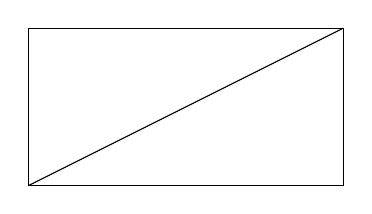
\begin{tikzpicture}[scale=10]
		\draw (0.0,0.0) rectangle (0.4,0.2);
		\draw (0.0,0.0) -- (0.4,0.2);
	\end{tikzpicture}\\
	\lipsum[1-3]
	\begin{figure}
		\centering
		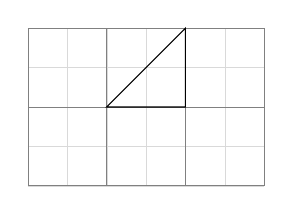
\begin{tikzpicture}
			\draw[line width=0.1pt,gray!30,step=5mm]
			(0,0) grid (3,2);
			\draw[help lines] (0,0) grid (3,2);
			\draw (1,1) -- (2,2) -- (2,1) -- cycle;
		\end{tikzpicture}
		\caption{Tikz Plot}
	\end{figure}

	\lipsum[1-3]
	

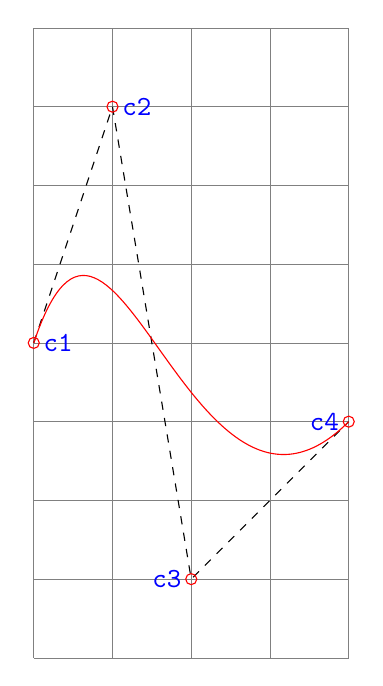
\begin{tikzpicture}
	\draw[help lines] (-2,-4) grid (+2,+4);
	\path (-2,+0) coordinate(c1)
	(-1,+3) coordinate(c2)
	(+0,-3) coordinate(c3)
	(+2,-1) coordinate(c4);
	\draw[dashed] (c1) -- (c2) -- (c3) -- (c4);
	\draw [color=red] (c1) circle (2pt)
	(c2) circle (2pt)
	(c3) circle (2pt)
	(c4) circle (2pt)
	(c1) .. controls (c2)
	and (c3) .. (c4);
	\draw [color=blue]
	(c1) node[anchor=west] {\texttt{c1}}
	(c2) node[anchor=west] {\texttt{c2}}
	(c3) node[anchor=east] {\texttt{c3}}
	(c4) node[anchor=east] {\texttt{c4}};
	
\end{tikzpicture}

	\lipsum[1]
	
	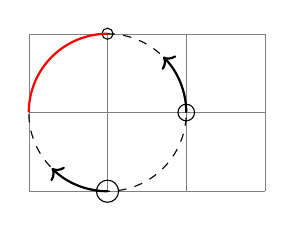
\begin{tikzpicture}
		\draw[help lines] (0,0) grid (3,2);
		\draw[dashed] (1,1) circle (1cm);
		\draw (1,2) coordinate(a) circle (2pt)
		(2,1) coordinate(b) circle (3pt)
		(1,0) coordinate(c) circle (4pt);
		\draw[color=red,-,thick] (a) arc (90:180:1cm);
		\draw[->,thick] (b) arc (0:45:1cm);
		\draw[->,thick] (c) arc (270:225:1cm);
	\end{tikzpicture}
	
	
	
	\lipsum[1]
	\subsection{Colour}
	\begin{tikzpicture}[color=red]
		\draw (0,3) -- (2,3);
		\draw[color=green, thick, ->] (0,2) -- (2,2);
		\draw[color=cyan!50!red] (0,1) -- (2,1);
	\end{tikzpicture}


\lipsum[1]


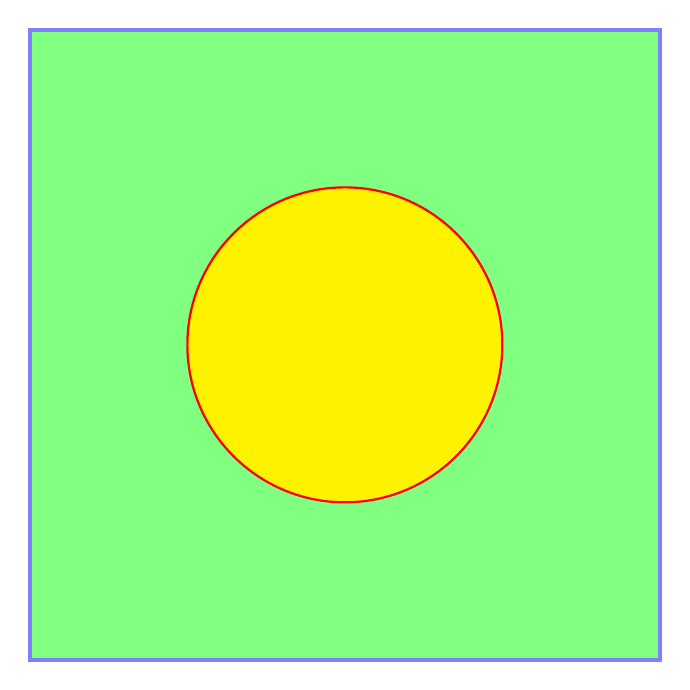
\begin{tikzpicture}[fill=blue!40,scale=4]
	\filldraw[ultra thick,fill=green!50, draw=blue!50]
	(0,0) rectangle (2,2);
	\filldraw[thick,fill=yellow,draw=red]
	(1,1) circle (0.5cm);
\end{tikzpicture}

\lipsum[1]

\begin{tikzpicture}
	\tikzstyle{connection}=[ultra thick,every node/.style={sloped,allow upside down},draw=\edgecolor,opacity=0.7]
	\node[canvas is zy plane at x=0] (temp) at (-3,0,0)
	 {\includegraphics[width=2cm,height=2cm]{1_1_09_2f_37.png}};
	
	\draw [color=black]
	 (temp) node[anchor=south] at (-3,-2){\texttt{Input Face}};
	%\draw[connection] 
	\draw[->,thick] (-2.5,0) -- (-2,0);
	
	\node[trapezium,
	draw = blue!80,
	text = black,
	fill = teal!20,
	rotate=270,
	trapezium stretches = true,
	minimum width = 2cm, 
	minimum height = 3cm] (t) at (-.5,0) {Feature Extraction};
	
	\draw[->,thick] (1.2,0) -- (1.7,0);
	
	\node[rectangle,
	draw = magenta!80,
	text = black,
	fill = magenta!20,
	rotate=270,
	trapezium stretches = true,
	minimum width = 2cm, 
	minimum height = 2cm] (t) at (3,0) {Classification};
	
	\pic[shift={(1.5,0,0)}] at (4,0) {Ball={name=elt1,%
			fill=\SumColor,opacity=0.6,%
			radius=3,logo=1/0?}};
		
\end{tikzpicture}







	
	
\end{document}
















